        
There is another kind of problem we care to work with.  All the problems we have considered have been initial value problems. However, there is a completely different type of problem we can solve.  This will be called a \boldgreen{boundary value problem}.  Let us make a comparison.

\subsubsection{Second Order Initial Value Problem}
\begin{itemize}
    \item Given a very general second order equation $x''=f(t,x,x')$ and initial data $x(0)=x_0$ and $x'(0)=v_0$.  
    \item Both conditions are given at the initial time $t=0$. We have one condition $x(0)$ for position and the other $x'(0)$ for velocity 
    \item Think of the solution $x(t)$ of tracking a particle over time. 
\end{itemize}

\subsubsection{Second Order Boundary Value Problem}
\begin{itemize}
    \item Given a very general second order equation $u''=f(x,u,u')$ and a \emph{region} $\Omega=[a,b]$ with \emph{boundary values} $u(a)=u_a$ and $u(b)=u_b$.
    \item Conditions are given at the endpoints of a region $\Omega=[a,b]$.  There will be one condition for every endpoint $a$, and $b$. The values will be given as $u(a)=u_a$ and $u(b)=u_b$. (\emph{Note: we may also prescribe slightly different conditions later on. These are referred to as Dirichlet boundary conditions.})
    \item Think of solution $u(x)$ as modeling a measurable quantity of an object (i.e., temperature, height, stress, or strain).
\end{itemize}

Boundary value problems are very important in the physical world.  For example, an engineer may wish to understand how a rod is deformed under the force of gravity as well as whatever machinery is pulling and pushing on it.  The engineer would hope to understand this deformation so that they can build sturdy structures.  In the field of chemistry, we see boundary value problems arise in thermal or quantum transport, in chemical reactions, in waves or lattice vibrations, and more. 

Not all boundary value problems are second order.  However, we'll concentrate first on problems that are second order as they are more pertinant for us.  The equations we'll start with will be Laplace's (or Poisson's) equation and then we'll move onto Schr\"odinger's equation.

\section{Laplace's and Poisson's Equations}

Let us set up the problem at hand.  We'll define our first boundary value problem as such.
\begin{df}{Boundary Value Problem}{boundary_val}
A \boldgreen{boundary value problem} is a differential equation (of possibly multiple variables) defined on a region in space $\Omega$ with prescribed \boldgreen{boundary data} (i.e., functions defined on the boundary of the region $\Omega$).  

For now, all regions will be $\Omega=[a,b]$, the \boldgreen{boundary} is the set $\{a,b\}$, and the differential equations will be second order.
\end{df}

\begin{remark}
Here, I will use the notation
\[
\frac{d}{dx}u=u'
\]
since we often like to think of $\frac{d}{dx}$ as an \emph{operator}.  We will get more into this later. Right now, it's just equivalent notation.
\end{remark}

\begin{ex}{Laplace's Equation: Dirichlet Boundary Data}{laplace}
\emph{Imagine a rod of length $L$ attached at endpoints $x=0$ and $x=L$.  The height of the endpoints of the rod are $u(0)=1$ and $u(L)=0$ respectively.  The rod is experiencing no external forces.  What is the shape of the rod?}\\

This problem statement leads us to consider the following boundary value problem
\[
\frac{d^2}{dx^2}u(x)=0
\]
on the region $\Omega = [0,L]$ with boundary data $u(0)=1$ and $u(L)=0$. Here, we are providing the function value that $u(x)$ must satisfy on the boundary.  Everywhere inside $\Omega$ (i.e., $(0,L)$), $u(x)$ must satisfy the differential equation as well. 

We know how to solve this equation as we can just integrate twice.  We find that the general solution is
\[
u(x)=C_1 x + C_2.
\]
We can solve for the constants $C_1$ and $C_2$ by using our boundary data. We require
\begin{align*}
    1&=u(0)=C_1(0)+C_2=C_2\\
    0&=u(L)=C_1(L)+C_2.
\end{align*}
The first equation gives us $C_2=1$ which we can plug into the second to get
\[
0=C_1(L)+C_2
\]
which means that $C_1=-\frac{1}{L}$.  Thus our particular solution to this boundary value problem is
\[
\boxed{u(x)=-\frac{1}{L}x+1.}
\]
\end{ex}

\begin{exercise}
Plot the above solution and verify it satisfies the ODE and the boundary values.  What can we say about the shape of the rod? Is is what we would expect?
\end{exercise}

So, the set up to these problems is a bit different, but solving them is fundamentally the same idea. Let's see some other examples of different equations.

\begin{df}{Laplace and Poisson Equations}{laplace_poisson}
On a region $\Omega=[a,b]$ we prescribe boundary data $u(a)=u_a$ and $u(b)=u_b$.  On this region, \boldgreen{Laplace's equation} is
\[
\frac{d^2}{dx^2}u(x)=0
\]
and \boldgreen{Poisson's equation} is 
\[
-\frac{d^2}{dx^2}(x)=F(x)
\]
for some given function $F(x)$. If this $F(x)$ is of the form $ku(x)$ for some constant $k$, then we have the equation for \boldgreen{eigenfunctions of the Laplacian}
\[
\frac{d^2}{dx^2}(x)=ku(x).
\]
We'll see that this equation shows up in quantum mechanics.
\end{df}

If we read the two examples and the definition of the Laplace and Poisson equations, we can get an intuition on what they're describing.  In a sense, both equations can describe the curvature of a 1-dimensional object.  Why is that? The second derivative gives us information about the curvature of a function at each point! For the Laplace equation, the curvature is said to be zero everywhere, hence when we integrated and found a solution, we found that we got a linear equation with some unknown coefficients that we could find with boundary data.  For the Poisson equation, however, there is some external force function $F(x)$ that deforms the rod.  So, the curvature should not be zero everywhere, which gives us a different set of solutions.  One may also notice that the solution to the Laplace equation appeared within the solution to the Poisson equation (go back and reread both to see this).  This is very much like solving homogeneous versus inhomogeneous second order linear ODEs with constant coefficients.

\begin{ex}{Poisson's Equation: Dirichlet Boundary Data}{poisson_neumann}
\emph{Consider a cable of length $1$ attached at endpoints $x=0$ and $x=1$.  Now, the attachment points of the cable is prescribed by specifying $u(0)=0$ and $u(1)=0$. The cable is also being pushed down by a constant force (like gravity). That is, $F(x)=-1$ constantly pulls the cable down.  We expect this cable to sag under this force much like power lines due under the force of gravity.}\\

This gives us the boundary value problem
\[
-\frac{d^2}{dx^2}(x)=-1
\]
on the region $\Omega = [0,1]$ with boundary data $u(0)=0$ and $u(1)=0$. We can integrate this equation twice to get
\[
u(x)= \frac{1}{2}x^2+bx+c.
\]
Now, we can use our boundary data to try and solve this problem. We require
\begin{align*}
    0=u(0)&=c,
\end{align*}
and hence $c=0$.  Thus, at this point we have $u(x)=\frac{1}{2}x^2+bx$.  The second equation from the second boundary value is then
\[
u(1)=\frac{1}{2}+b,
\]
and so $b=-\frac{1}{2}$. Hence our particular solution to the boundary value problem is
\[
\boxed{u(x)=\frac{1}{2}x^2-\frac{1}{2}x.}
\]
We can plot this solution and see if this makes physical sense.
\begin{figure}[H]
    \centering 
    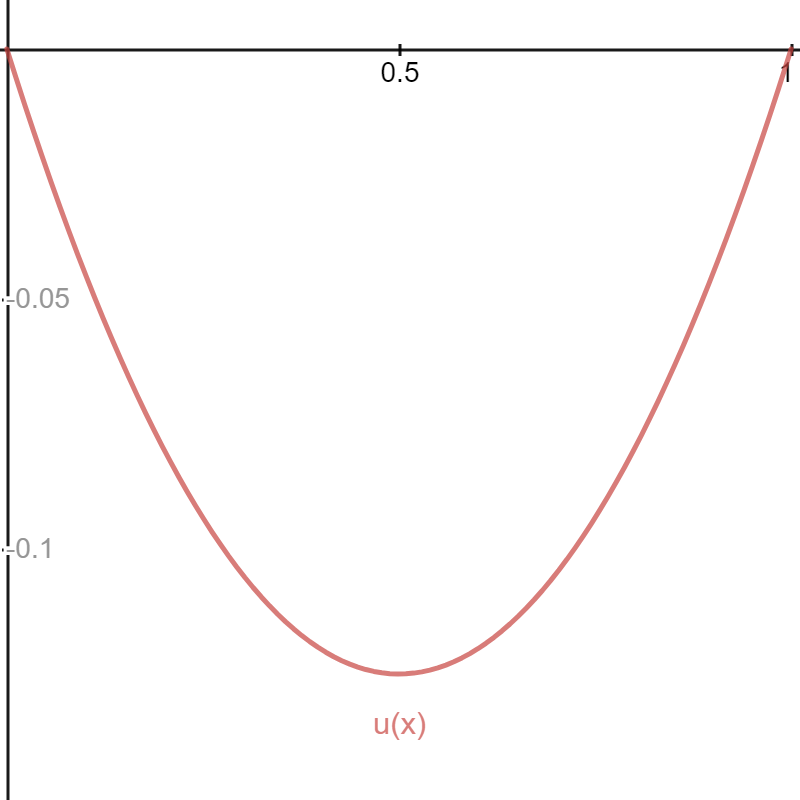
\includegraphics[width=.6\textwidth]{Figures_Part_1/poisson_equation_gravity.png}
    \caption{The profile of a cable under a constant force directed downward.}
\end{figure}

It seems like the curvature of this cable is close to what we would expect.  How much deformation there is would depend on the strength of the force $F(x)$ as well as the elastic properties of the cable.  These would all factor in to the equation if we considered it in greater detail.
\end{ex}

\section{A Particle in a 1-Dimensional Box}

Now, let's enter into some quantum mechanics.  In essence, quantum mechanics is governed by the \emph{Schr\"odinger equation}.  Think of this equation as a quantum version of Newton's laws.  Right now, we have only considered ODEs, and as such we will consider a particular case of Sch\"odinger's equation which is independent of time. The \boldgreen{time independent Schr\"odinger  equation} describes a \boldgreen{stationary state} of a particle which we denote by $\psi(x)$.  If we put $\psi(x)$, we are thinking of this particle as not evolving in time, but having this function describing its position nonetheless.  In general, we call a function $\Psi(x,t)$ that solves time dependent version of Schr\"odinger's equation a \boldgreen{wavefunction}. Again, we will not approach the time dependent portion until we reach the sequel of this course.  A wavefunction is not quite physically meaningful in its own right.  However, it gives rise to a probability interpretation of the particle. We'll see that shortly.

\begin{df}{Time Independent Schr\"odinger Equation}{time_ind_schro}
The \boldgreen{one dimensional time independent Schr\"odinger equation} with \boldgreen{potential} $V(x)$ is given by the differential equation
\[
\left(-\frac{\hbar^2}{2m}\frac{d^2}{dx^2}+V(x)\right)\Psi(x)=E\Psi(x).
\]
Here, $\Psi$ is the wavefunction and in this case we will only find that the allowed wavefunctions can only be stationary states. $\hbar$ is a physical constant called \boldgreen{Planck's reduced constant}, $E$ is the energy, and $m$ is the mass of what ever particle we are considering at the moment. Note that $E$ is not fixed in this equation and is taken to be an unknown parameter (until we solve the equation). The quantity
\[
-\frac{\hbar^2}{2m}\frac{d^2}{dx^2}+V(x)
\]
is called the \boldgreen{Hamiltonian operator}.
\end{df}

If we think of a particle in a 1-dimensional box of length $L$, then the region the particle can exist is $[0,L]$.  We're making it impossible for the particle to leave this box and we can do that using the potential $V(x)$. If we assign
\[
V(x)=\begin{cases} 0 & \textrm{if } 0<x<L\\
\infty & \textrm{if } x\leq 0 ~\textrm{or}~ x\geq L. \end{cases}.
\]
This gives rise to the boundary value problem
\[
-\frac{\hbar^2}{2m}\frac{d^2\Psi}{dx^2}=E\psi
\]
with boundary conditions $\Psi(0)=0$ and $\Psi(L)=0$. This should look much like the eigenfunction equation for the Laplacian we saw previously. These boundary conditions will seem more sensible when we get a better interpretation of the wavefunction $\Psi$. If you'd like, you can essentially plug in $V(x)=\infty$ and see that the only possibility for a solution is that $\Psi(x)=0$ (but this is a bit handwavy). 

Now, let us solve this boundary value problem.  We have a second order linear differential equation with constant coefficients. In fact, it is also homogeneous as we can write 
\[
\frac{d^2\Psi}{dx^2}+\frac{2mE}{\hbar^2}\Psi =0.
\]
Now, to solve this, find roots $\lambda_1$ and $\lambda_2$ to the characteristic polynomial
\[
\lambda^2+\frac{2mE}{\hbar^2}=0.
\]
We solve this by letting $\omega^2 = \frac{2mE}{\hbar^2}$ and putting
\begin{align*}
    \lambda^2&=-\omega^2\\
    \lambda&=\pm i \omega,
\end{align*}
so $\lambda_1=i\omega$ and $\lambda_2=\lambda_1^*$. This then gives us the general solution
\[
\Psi(x)=C_1 e^{i\omega x}+C_2 e^{-i\omega x}.
\]
Of course, it is also possible to write 
\[
\Psi(x)=C_1\cos(\omega x)+C_2\sin(\omega x),
\]
as this is just an equivalent way to write out the general solution. Now, we have our boundary conditions $\Psi(0)=0$ and $\Psi(L)=0$ as well.  Plugging these into our general solution gives us
\begin{align*}
    0=\Psi(0)&=C_1 \cos(\omega \cdot 0)+C_2 \sin(\omega \cdot 0)\\
    &= C_1,
\end{align*}
so $C_1=0$.  Next, we have
\begin{align*}
    0=\Psi(L)&=C_2\sin(\omega \cdot L).
\end{align*}
Now, how are we to solve this equation? We must have that input to the sin function must be an integer $n=\dots,-2,-1,0,1,2,\dots$ copy of $\pi$ as $\sin(n\pi)=0$. Else, we force $C_2=0$ which gives us nothing!  So, we require
\[
\omega L = n\pi.
\]
Recall that $\omega = \frac{2mE}{\hbar^2}$ and that $E$ is not determined (yet)! So now we have that $\omega = \frac{n\pi}{L}$ which gives us a general solution we will denote with a subscript $n$
\[
C\psi_n(x)=\sin\left(\frac{n\pi x}{L}\right).
\]
Note that I have changed the constant just to $C$ on $\psi_n$, and we'll solve for this constant soon enough.  For each solution $\psi_n$ there corresponds an energy $E_n$ that we can solve for by
\begin{align*}
    \omega_n^2  &= \left(\frac{n \pi}{L}\right)^2\\
    \frac{2mE_n}{\hbar^2}&= \left(\frac{n\pi}{L}\right)^2,
\end{align*}
which when we solve for $E_n$ gives us
\[
   \boxed{E_n = \frac{n^2\hbar^2\pi^2}{2mL}.}
\]
What have we found? We have found that to each solution $\psi_n$ there corresponds an energy value $E_n$. We've also seen that there are infinitely many solutions but they correspond to \boldgreen{quantized} energy levels! We can disregard some of our solutions as well. In fact, we keep only $n=1,2,3,\dots$ as $n=0$ gives us $\psi_0(x)=0$ which is not a physical solution (we'll see more on this in just a bit).  Also, we have that $\psi_n(x)=-\psi_{-n}(x)$, so the negative values for $n$ are simply redundant.

The interpretation of the $\psi_n$ is that they are the allowable \boldgreen{stationary states}\index{states!stationary} of the system. In this case, the system is the particle in a 1-dimensional box. In general, a \boldgreen{wavefunction}\index{wavefunction} $\Psi(x,t)$ will be a sum of these states, but with an added time dependence that we did not talk about here. The wavefunction describes a \boldgreen{probability} of a particle being at a position.  How so? Well, the following integral gives us the probability (a number $P\in [0,1]$) of a particle with a wavefunction $\Psi(x,t)$ being the region $[a,b]$.  
\[
P([a,b]=\int_a^b |\Psi(x,t)|^2 dx=\int_a^b \Psi^* \Psi dx,
\]
where $|\Psi(x,t) |$ represents the modulus of the complex wavefunction $\Psi(x,t)$. This interpretation of quantum mechanics is just another part of what makes the theory so different from classical theory! We can only make predictions in a probabalistic way! Truly, it's fascinating. Keep in mind, we really can only do this for the initial profile $\Psi(x,0)$ since we have not introduced time dependence just yet.

In order to have this integral give us a valid probability at time $t=0$, we must \boldgreen{normalize} the stationary states $\psi_n(x)$ by requiring that
\[
\int_{-\infty}^\infty |C\psi_n(x)|^2dx=1.
\]
We can compute this explicitly by finding $C$. So we have for the particle in a 1-dimensional box,
\begin{align*}
    1&= \int_{-\infty}^\infty |C\psi_n(x)|^2dx\\
    &= C^2\int_{0}^L \sin^2\left(\frac{n\pi x}{L}\right)dx \qquad \textrm{since $\psi_n=0$ outside of $[0,L]$}\\
    &= C^2 \frac{L}{2}
\end{align*}
which gives us that the \boldgreen{normalization constant} $C=\sqrt{\frac{2}{L}}$ for any state $\psi_n$. So the normalized stationary states of the system are then
\[
\boxed{\psi_n(x) = \sqrt{\frac{2}{L}}\sin\left(\frac{n\pi x}{L}\right).}
\]

In general, one would hope to combine our states to create a more general wavefunction as
\[
\Psi(x) = \sum_{j=1}^\infty a_j \psi_j.
\]
We refer to this $\Psi(x)$ as a superposition of states.  Without adding in time dependence, it is \textbf{not} true that a superposition of states solves the time independent Schr\"odinger equation! 

Next, we can consider the \boldgreen{inner product}\index{inner product} between states $\psi_n$ and $\psi_m$ which tells us how much of each state ``points in the same direction"
\[
\langle \psi_n,\psi_m \rangle \coloneqq \int_{\infty}^\infty \psi_n^*(x) \psi_m(x) dx.
\]
If we evaluate this integral, we find that
\begin{align*}
    \int_{-\infty}^\infty \psi_n^*(x)\psi_m(x)dx&= \frac{2}{L}\int_0^L \sin\left( \frac{n\pi x}{L}\right)\sin\left( \frac{m\pi x}{L}\right)dx\\
    &= \begin{cases} 0 &\textrm{if}~ n\neq m\\
    1 & \textrm{if}~ n=m\end{cases}.
\end{align*}
Sometimes we denote this by putting
\[
\langle \psi_n,\psi_m\rangle = \delta_{nm}
\]
and saying that the $\psi_n$ are \boldgreen{orthogonal}\index{orthogonal}. In fact they are even \boldgreen{orthonormal}\index{orthonormal} since
\[
\langle \psi_n,\psi_n\rangle = 1,
\]
since we have normalized each state.
\begin{exercise}
Evaluate the above integral for $\langle \psi_n, \psi_m \rangle$ to show that you get $\langle \psi_n,\psi_m\rangle = \delta_{nm}$.  \emph{Hint: use the following substitution} 
\[
\sin\left(\frac{n\pi x}{L}\right)\sin\left(\frac{n\pi x}{L}\right) =\frac{1}{2}\left[ \cos\left( \frac{(n-m)\pi x}{L} \right) - \cos\left( \frac{(m+n)\pi x}{L}\right)\right].
\]
\end{exercise}
What do these states of the system look like? We can plot them for different values of $n$. Let's take a look. Here we will let $L=1$ for the plots.
        \begin{figure}[H]
    \centering
    \begin{subfigure}[h]{0.3\textwidth}
        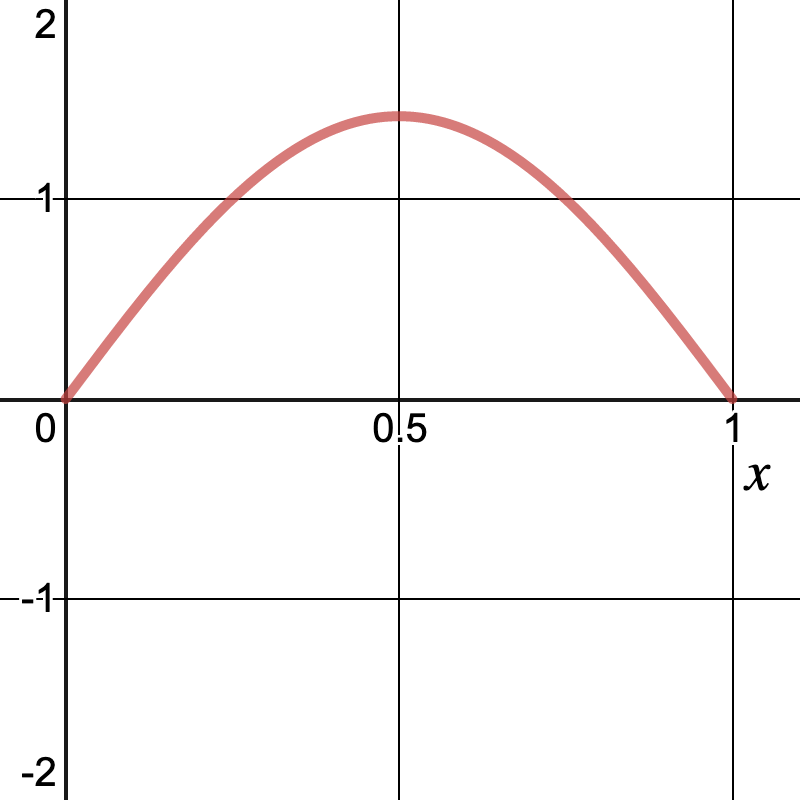
\includegraphics[width=\textwidth]{Figures_Part_2/state_1.png}
        \caption{$\psi_1(x)$.}
    \end{subfigure}
    ~ 
    \begin{subfigure}[h]{0.3\textwidth}
        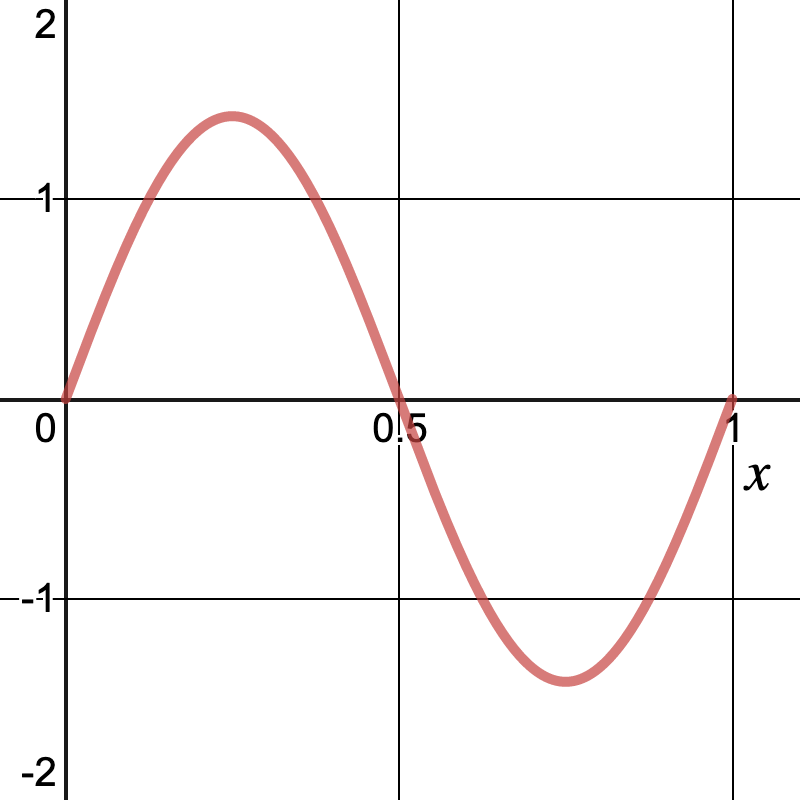
\includegraphics[width=\textwidth]{Figures_Part_2/state_2.png}
        \caption{$\psi_2(x)$.}
    \end{subfigure}
    ~
    \begin{subfigure}[h]{0.3\textwidth}
        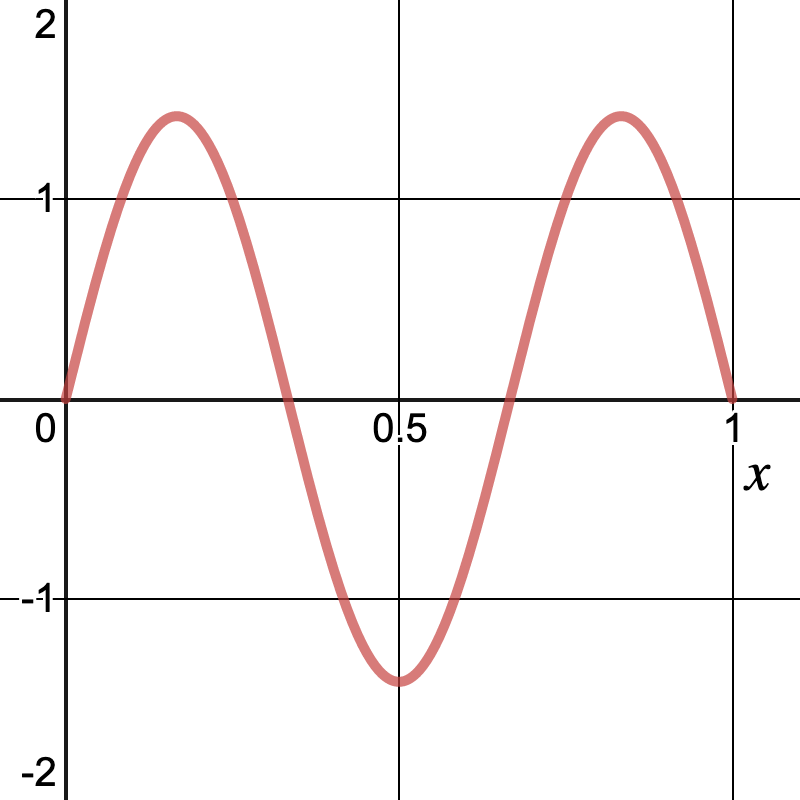
\includegraphics[width=\textwidth]{Figures_Part_2/state_3.png}
        \caption{$\psi_3(x)$.}
    \end{subfigure}\\
    
        \begin{subfigure}[h]{0.3\textwidth}
        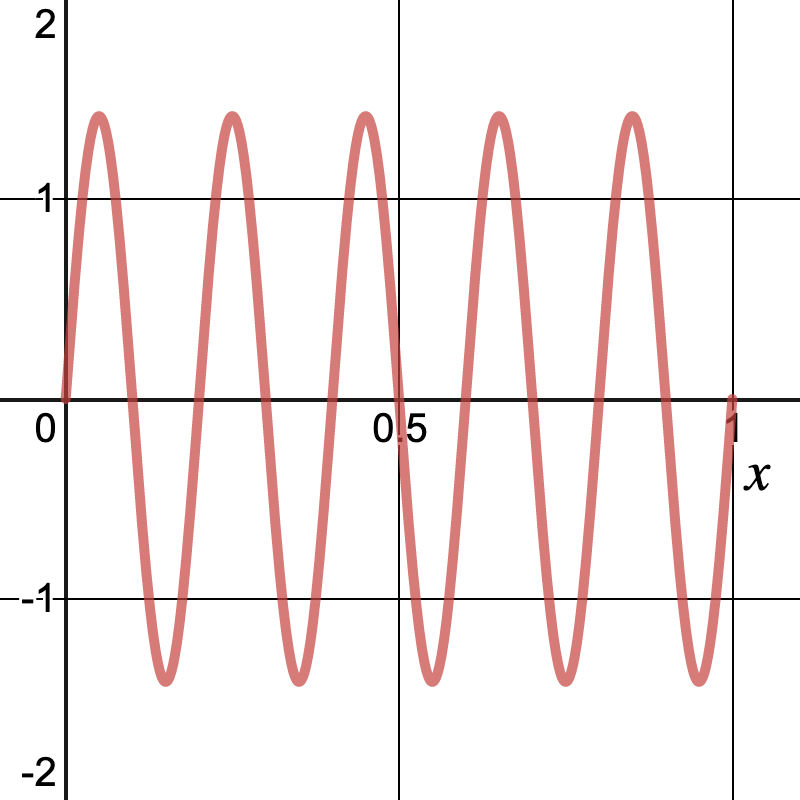
\includegraphics[width=\textwidth]{Figures_Part_2/state_10.png}
        \caption{$\psi_{10}(x)$.}
    \end{subfigure}
    ~ 
    \begin{subfigure}[h]{0.3\textwidth}
        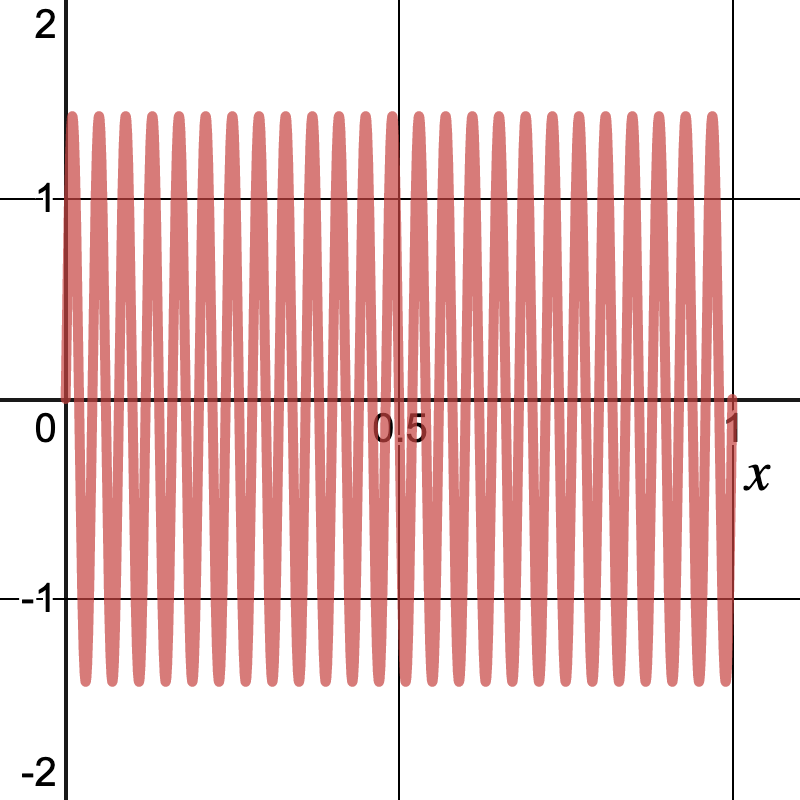
\includegraphics[width=\textwidth]{Figures_Part_2/state_50.png}
        \caption{$\psi_{50}(x)$.}
    \end{subfigure}
    ~
    \begin{subfigure}[h]{0.3\textwidth}
        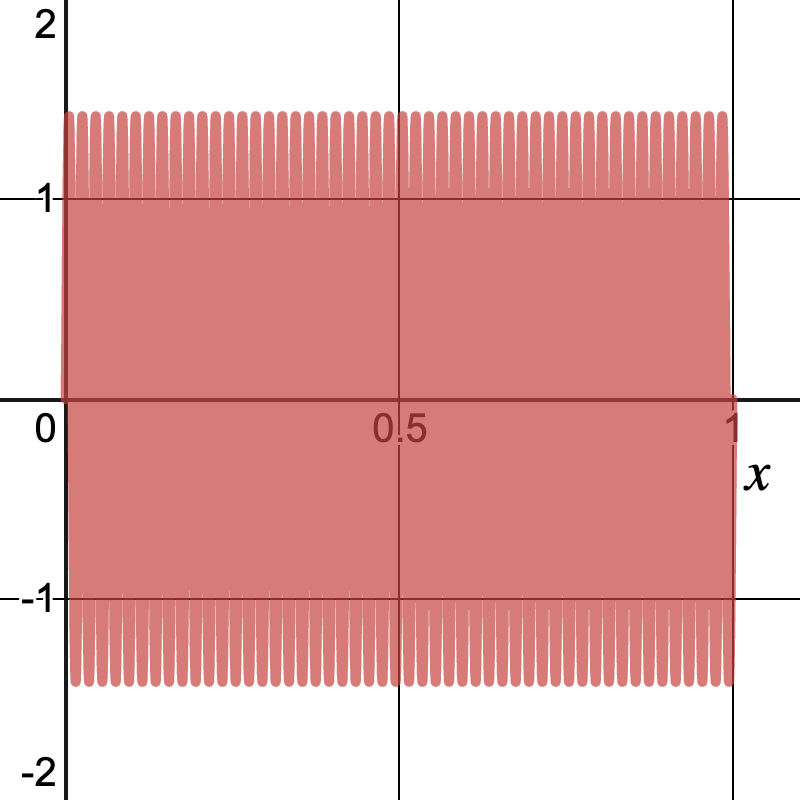
\includegraphics[width=\textwidth]{Figures_Part_2/state_100.png}
        \caption{$\psi_{100}(x)$.}
    \end{subfigure}
        \end{figure}

\noindent One may notice that as we allow for larger and larger $n$ values, the states seem to start to approach a uniform value on the region $[0,L]$. In fact, if we were to take the limit as $n\to \infty$, we would essentially have that $\psi_\infty(x) = \frac{1}{L}$ which would be equivalent to the case of a classic particle randomly placed in the box.

When we add in time dependence, it is possible to prepare this system in a \boldgreen{superposition} by, for example, considering the wavefunction
\[
\Psi(x,0) = \frac{1}{\sqrt{2}}\left(\psi_1(x) + \psi_2(x)\right).
\]
More generally, due to the orthonormality of the stationary states, we can write a wavefunction $\Psi(x,0)$ as
\[
\boxed{\Psi(x,0)=\sum_{j=1}^\infty a_j \psi_j(x) \qquad \textrm{where}\qquad \sum_{j=1}^\infty a_j^2 = 1.}
\]

\subsubsection{Summary of the 1-Dimensional Box}
\begin{itemize}
    \item The equation for the 1-Dimensional box is the same as the eigenfunctions of the Laplacian equation shown before. That is, we have $V(x)=0$ and we allow for $x$ to be in the range $[0,L]$ and get the equation
    \begin{align*}
        H\Psi &= E \Psi\\
        -\frac{\hbar^2}{2m}\frac{d^2}{dx^2}\Psi = E \Psi.
    \end{align*}
    \item We solved this equation as a second order linear equation and used the boundary values to determine possible solutions.  It turns out that we get a quantized set of solutions $\psi_n$ each corresponding to an energy level $E_n$. These energy levels were given by $E_n = \frac{n^2 \hbar^2 \pi^2}{2mL}$ and so the energies increase proportionally to $n^2$. We can see a plot of energies here.
    \begin{figure}[H]
        \centering
        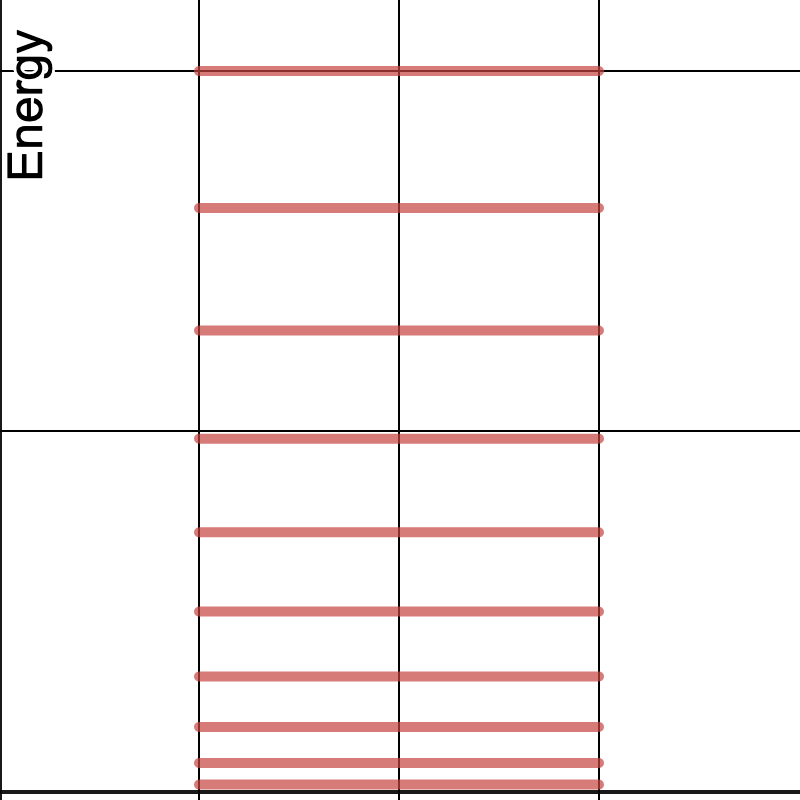
\includegraphics[width=.5\textwidth]{Figures_Part_2/energy_levels.png}
        \caption{Energy levels of the 1-dimensional box.}
    \end{figure}
    \item We normalized the solutions $\psi_n$ and found that they give rise to a probability function that describe the probability of a particle being in a region $[a,b]$. 
    \item We can take an initial profile for a wavefunction as a superposition
    \[
    \Psi(x,0)=\sum_{j=1}^\infty a_j \psi_j(x)
    \]
    where $\sum_{j=1}^\infty a_j^2 = 1$. If more than one $a_j\neq 0$, then this wavefunction describes a superposition state. 
    \item We can then find the probability of a particle with wavefunction $\Psi(x,t)$ being in the region $[a,b]$ at time $t$ by
    \[
    P([a,b])=\int_a^b |\Psi(x,t)|^2dx.
    \]
    To do this to the full extent, we do need to add in time dependence which we do not consider at this moment! However, alluding to what we wrote for $\Psi(x,0)$, we can compute this probability for a superposition of states $\psi_n$ at time $t=0$.
    \item As we let $n\to \infty$, we recover the case of the classical particle.  We should expect this since we do not observe this odd quantum phenomenon on large scale!
\end{itemize}

\begin{exercise}
Look up common energies for something like throwing a baseball. Compare this to $E_n$ for $m=1[g]$ and $L=1[m]$. You will have to use the measured value for Planck's reduced constant
\[
\hbar \approx 1.0545718\cdot 10^{-34}[kg \cdot m^2 /s].
\]
\end{exercise}

\begin{remark}
    The time dependent aspect will be covered after we learn multivariate calculus in Math 272.  There we will find that superposition of time dependent states does indeed give us a solution to the time dependent version of the equation.  
\end{remark}

